\documentclass{article}
\usepackage[a4paper, margin=1in]{geometry} % Adjust margin size as needed
\usepackage{graphicx} % Required for inserting images
\usepackage{listings}
\lstset{basicstyle=\ttfamily}
\usepackage{float}
\usepackage{courier}
\usepackage{tabularx}
\usepackage{tikz}
\usepackage{url}
\usepackage{amsmath}
\usepackage{float}
\usepackage{hyperref}
\usepackage{MnSymbol}
\usepackage{indentfirst}

\title{Concepts of Programming - Project \#1: Parser}
\author{Daniel Marin and Jennifer Vicentes}
\date{October 22$^{nd}$, 2024}

\begin{document}
\maketitle
\tableofcontents
\newpage
\section{Introduction}
\subsection{Context}
For the 2$^{nd}$ deliverable of this project we where expected to create a parser that does not compute the notes that make up the chords. For the elaboration of this section of the project we used the following grammar and sets to help as a guide when coding this parser:
\subsubsection{Grammar Rules}
\begin{figure}[H]
    \centering
    \begin{lstlisting}
      input:=  song EOF
       song:=  bar {bar} "|"
        bar:=  [meter] chords "|"
      meter:=  numerator "/" denominator
  numerator:=  "1" | "2" | "3" | ... | "15"
denominator:=  "1" | "2" | "4" | "8" | "16"
     chords:=  "NC" | "%" | chord {chord}
      chord:=  root [description] [bass]
       root:=  note
       note:=  letter [acc]
     letter:=  "A" | "B" | "C" | ... | "G" |
description:=  qual | qual qnum | qnum | qnum sus | sus
       qual:=  "-" | "+" | "o"
       qnum:=  ["^"] num
        num:=  "7" | "9" | "11" | "13"
        sus:=  "sus2" | "sus4"
       bass:=  "/" note
        acc:=  "b" | "#"
    \end{lstlisting}
    \caption{Chords Grammar. The input consists of the chords in a song separated by bar lines "$|$" plus optional meter information for the bars. (This grammar is a subset of the grammar used by Polynizer: \url{https://www.polynizer.com})}
    \label{fig:Grammar}
\end{figure} 
All grammar related functions in 'Parser.c' are an interpretation of the grammar rules shown in figure \ref*{fig:Grammar}. With the use of the concepts seen in class and in the book. Also, as mentioned before here we have the first and follow sets of this grammar from deliverable one of this project.
\subsubsection{First and Follow Sets of Grammar}
\begin{figure}[H]
    \def\arraystretch{1.5}%
    \begin{tabularx}{\textwidth}{l|X|X}
        Nonterminal & First set & Follow set \\
        \hline
        \hline
        \lstinline|input| & \{1, 2, 3, 4, 5, \ldots, 15, \%, \texttt{NC}, A, B, C, D, E, F, G\} & \{\}\\
        \hline
        \lstinline|song| & \{1, 2, 3, 4, 5, \ldots, 15, \%, \texttt{NC}, A, B, C, D, E, F, G\} & \{\texttt{EOF}\}\\
        \hline
        \lstinline|bar| & \{1, 2, 3, 4, 5, \ldots, 15, \%, \texttt{NC}, A, B, C, D, E, F, G\} & \{ $\vert$, 1, 2, 3, 4, 5, \ldots, 15\} \\
        \hline
        \lstinline|meter| &  \{1, 2, 3, 4, 5, \ldots, 15\} 
        & \{\%, \texttt{NC}, A, B, C, D, E, F, G\} \\
        \hline
        \lstinline|numerator| & \{1, 2, 3, 4, 5, \ldots, 15\} 
        & \{ /\}\\
        \hline
        \lstinline|denominator| & \{1, 2, 4, 8, 16\} 
        & \{\%, \texttt{NC}, A, B, C, D, E, F, G\} \\
        \hline
        \lstinline|chords| & \{\%, \texttt{NC}, A, B, C, D, E, F, G\}
        & \{ $\vert$ \} \\
        \hline
        \lstinline|chord| & \{A, B, C, D, E, F, G\}  & 
        \{ $\vert$, A, B, C, D, E, F, G\} \\
        \hline
        \lstinline|root| & \{A, B, C, D, E, F, G\} 
        & \{-, +, o, \lstinline|^|, 7, 9, 11, 13, \texttt{sus2}, \texttt{sus4}, /, $\vert$, A, B, C, D, E, F, G\} \\
        \hline
        \lstinline|note| & \{A, B, C, D, E, F, G\} 
        & \{-, +, o, \lstinline|^|, 7, 9, 11, 13, \texttt{sus2}, \texttt{sus4}, /, $\vert$, A, B, C, D, E, F, G\} \\
        \hline
        \lstinline|letter| & \{A, B, C, D, E, F, G\} 
        & \{\#, b, -, +, o, \lstinline|^|, 7, 9, 11, 13, \texttt{sus2}, \texttt{sus4}, /, $\vert$, A, B, C, D, E, F, G\} \\
        \hline
        \lstinline|description| & \{-, +, o, \lstinline|^|, 7, 9, 11, 13, \texttt{sus2}, \texttt{sus4}\}  & \{/, $\vert$, A, B, C, D, E, F, G\} \\
        \hline
        \lstinline|qual| & \{-, +, o\} 
        & \{/, $\vert$, A, B, C, D, E, F, G,\lstinline|^|, 7, 9, 11, 13\} \\
        \hline
        \lstinline|qnum| & \{\lstinline|^|, 7, 9, 11, 13\}  & \{/, $\vert$, A, B, C, D, E, F, G, \texttt{sus2}, \texttt{sus4}\}  \\
        \hline
        \lstinline|num| & \{7, 9, 11, 13\} 
        & \{/, $\vert$, A, B, C, D, E, F, G, \texttt{sus2}, \texttt{sus4}\} \\
        \hline
        \lstinline|sus| & \{\texttt{sus2}, \texttt{sus4}\} 
        & \{/, $\vert$, A, B, C, D, E, F, G\}  \\
        \hline
        \lstinline|bass| & \{/\} 
        & \{ $\vert$, A, B, C, D, E, F, G\}\\
        \hline
        \lstinline|acc| & \{\#, b\} 
        & \{-, +, o, \lstinline|^|, 7, 9, 11, 13, \texttt{sus2}, \texttt{sus4}, /, $\vert$, A, B, C, D, E, F, G\} \\
        \hline
    \end{tabularx}
    \caption{First and Follow Sets of the Grammar in figure \ref*{fig:Grammar} developed in deliverable 1.}
    \label{fig:FirstAndFollowSets}
\end{figure}
Figure \ref*{fig:Grammar} and \ref*{fig:FirstAndFollowSets} helped us develop the flow of the program and it's elaboration in a concise but proper manner. This report document focuses on explaining each function, the tests that where performed to prove functionality.
\subsection{Usage}
The usage of this program is fairly easy. To use this program as of the current state of this folder you must first add a song as a \texttt{.txt} file to the \textbf{Songs} folder. Run the program, when prompted "\texttt{Enter the path of the file to be parsed:}" copy the file path.
\subsection{Platform}
The development of this project was all done in C with the help of the grammar rules and Chapter 6.6 - Parsing Techniques and Tools from Programming Languages - Kenneth C. Louden - 3ed.
\section{Functions} \label{fig:Functions}

\subsection{Main}
The main function is fairly straightforward it is in charge of setting up the parser by following the next steps:
\begin{itemize}
    \item Getting the filepath from the user, preferrebly one that uses the Songs folder.
    \item Determining if the type of file is supported and if it can be opened, if the file is a '.txt', proceed to parse, if not exit program. 
    \item Parse the contents of the '.txt', if the contents are correct according to the grammar it should print them without the spaces.
\end{itemize}
To better comprehend this behavior, following is the code of the main function. 
\begin{figure}[H]
    \begin{lstlisting}[language=C]
int main(void){
    char filepath[365];
    printf("Enter the path of the file to be parsed: ");
    scanf("%[^\n]s", filepath);
    if (strlen(filepath) < 4 || 
        strcmp(filepath + strlen(filepath) - 4, ".txt") != 0) {
        printf("Error: Only .txt files are supported\n");
        exit(1);
    }
    inputFile = fopen(filepath, "r");
    if (inputFile == NULL){
        printf("Error: cannot open file\n");
        exit(1);
    }
    printf("The following characters demonstrate the tokens being parsed.\n\n");
    getToken();         // initiates the file reading 
    input();
    printf("\n");
    printf("\nParsing completed successfully\n");
    fclose(inputFile);
    return 0;
}
    \end{lstlisting}
    \caption{Uncommented \texttt{main} function from Parser.c}
\end{figure}
\subsection{Parsing Functions}
This section contains the functions that aren't grammar dependant and can be used whenever needed for parsing a '.txt' file.
\subsubsection{\texttt{void error(char *message)}}
This function is at simple as it gets, whenever called it is supposed to print out a message for the user to see whenever there is an error, and exit the program. In this program it is primarily used to catch parsing errors and prevent them from propagating later on.
\begin{figure}[H]
    \begin{lstlisting}[language=C]
void error(char* message) {
    printf("\nParse error: %s\n", message);
    exit(1);
}
    \end{lstlisting}
    \caption{Uncommented \texttt{error} function from Parser.c}
\end{figure}

\subsubsection{\texttt{void getToken()}}
This function is in charge of retrieving the next token to be parsed whenever it is called, ignoring newlines, tabulars and spaces. Thus retrieving possibly parsable tokens from the file.
\begin{figure}[H]
    \begin{lstlisting}[language=C]
void getToken(){
    token = getc(inputFile);
    if (token == EOF) return; 
    while(token == ' ' || token == '\n' || token == '\t'){
        token = getc(inputFile);
    }
}
    \end{lstlisting}
    \caption{Uncommented \texttt{getToken} function from Parser.c}
\end{figure}
\subsubsection{\texttt{void match(char c, char* message)}} 
This function is simple, it is a controller that is in charge of deciding whether the current token is the desired character and we should prompt the \texttt{getToken()} function, or if there was an error parsing and it should prompt an \texttt{error(message)}.
\begin{figure}[H]
    \begin{lstlisting}[language=C]
void match(char c, char* message){
    if (token == c) 
        getToken();
    else 
        error(message);
}
    \end{lstlisting}
    \caption{Uncommented \texttt{match} function from Parser.c}
\end{figure}
\subsection{Grammar Functions}
This section contains all the grammar dependant functions used in the development of this parser. They are what trully parse the contents of the document with the help of the functions in the Parsing Functions Section.
\begin{itemize}
    \item \textbf{Rule 1:} \texttt{void input()} - is in charge of initializing the parsing of the song and matching the EOF character. Basically, starting and ending the the parsing.
    \item \textbf{Rule 2:} \texttt{void song()} - is in charge of parsing the structure of the song, by parsing bars until it encounters a '|' after any bar, insinuating that the song has been completely parsed.
    \item \textbf{Rule 3:} \texttt{void bar()} - is in charge of parsing the structure of a bar, checking for the optional meter by asking if the token is a digit. The parsing the chords, and finally matching the '|' character.
    \item \textbf{Rule 4:} \texttt{void meter()} - is in charge of parsing the structure of a meter, first retrieving a numerator, matching the '/' and finally retrieving the denominator.
    \item \textbf{Rule 5:} \texttt{int numerator()} - is in charge of checking if the numerator is in the valid range (from 1 - 15), and then returning if valid. Else, it should prompt an error. 
    \item \textbf{Rule 6:} \texttt{int denominator()} - is in charge of checking if the denominator is a valid one (denominator $\in$ [1,2,4,8,16]), and returning if so. Else, it should prompt an error.
    \item \textbf{Rule 7:} \texttt{void chords()} - is in charge of parsing the structure of a set of chords by either checking for the "\texttt{NC}" or the "\texttt{\%}" token, or checking for repeated set of chord. 
    \item \textbf{Rule 8:} \texttt{void chord()} - is in charge of parsing the structure of a chord by calling \texttt{root} and checking if the chord contains a description and a bass.
    \item \textbf{Rule 9:} \texttt{void root()} - is in charge of calling note and is placed here since it will help us represent the notes in deliverable 3, by separating a root from a bass.
    \item \textbf{Rule 10:} \texttt{void note()} - is in charge of parsing the structure of a note by calling \texttt{letter} function and then checking if it should call the \texttt{acc} function.
    \item \textbf{Rule 11:} \texttt{char letter()} - is in charge of checking if the letter is a valid one ([A-G]), and returning it for the note to parse.
    \item \textbf{Rule 12:} \texttt{char acc()} - is in charge of checking if the accent is a valid one (either \# or b).
    \item \textbf{Rule 13:} \texttt{void description()} - is in charge of checking which of the optional description has by using a set of dedicated combinations seen in this rule. Anything else, should prompt an error.
    \item \textbf{Rule 14:} \texttt{char qual()} - is in charge of checking if the quality of the chord is the correct one (either -,+,o). 
    \item \textbf{Rule 15:} \texttt{void qnum()} - is in charge of checking for valid combinations of a qnum and a num (options are a \texttt{\^{}} symbol and a num or a num).
    \item \textbf{Rule 16:} \texttt{int num()} - is in charge of checking using the same method as the numerator for a valid number $\in$ [7,9,11,13]. This returns it also or prompts an error.
    \item \textbf{Rule 17:} \texttt{void sus()} - is in charge of checking if the suspension is either $sus2$ or $sus4$.
    \item \textbf{Rule 18:} \texttt{void bass()} - is in charge of parsing the structure of a bass by matching the '/' and prompting the \texttt{note} function.
\end{itemize}
\indent Some of these functions have added functionality to print certain results for the user of the program to actually visualize the characters being parsed and the order of execution.
\section{Test and Results} \label{fig:Results}
The tests for the program are all the '.txt' files posted by Dr. Arturo Camacho on blackboard, they are songs parsed using Polynizer app\footnote{Polynizer app link: \url{https://www.polynizer.com}} which are just a set of terminals/tokens bundled in a neatly organized manner, that when played create a song. Those tests are encompassed by the following itemize, which are the files in the Songs folder and their respective results. 
\begin{itemize}
    \item \textbf{Test 1}: Bruno Mars, Anderson Paak, Silk Sonic - Skate.txt
    \begin{figure}[H]
        \centering
        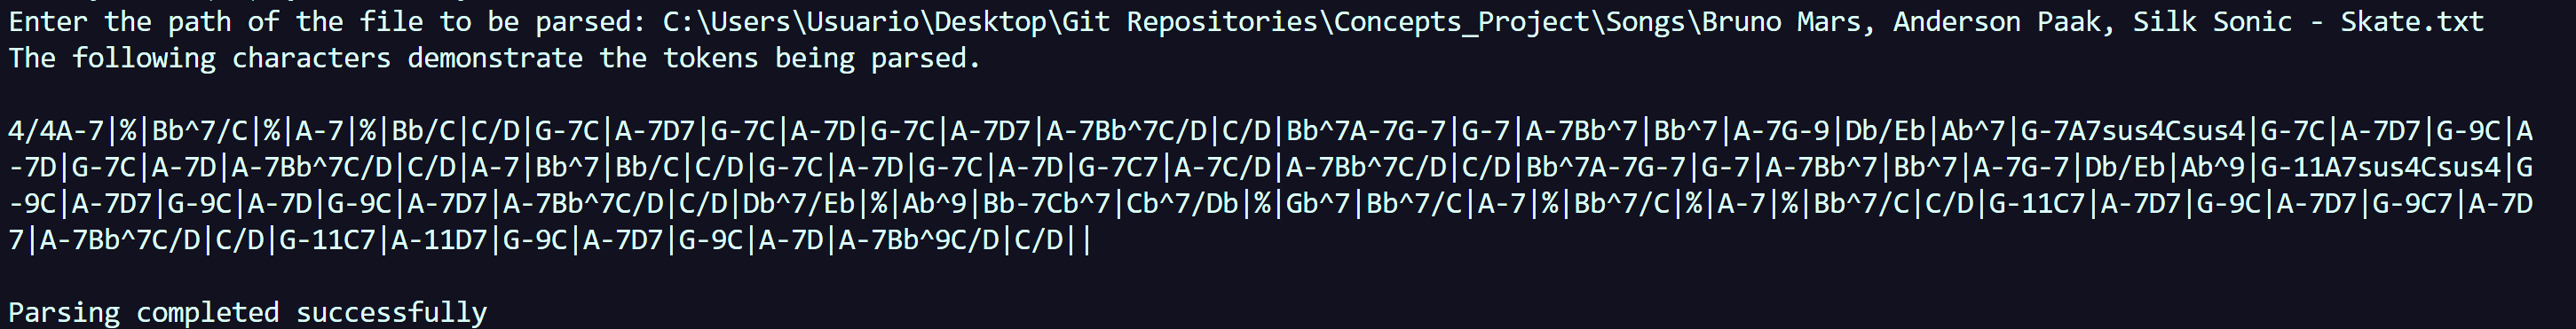
\includegraphics[width=1\textwidth]{Image_SkateParsed.png}
        \caption{Image of outputs on the command line.}
    \end{figure}
    \item \textbf{Test 2}: John Legend - All of me.txt
    \begin{figure}[H]
        \centering
        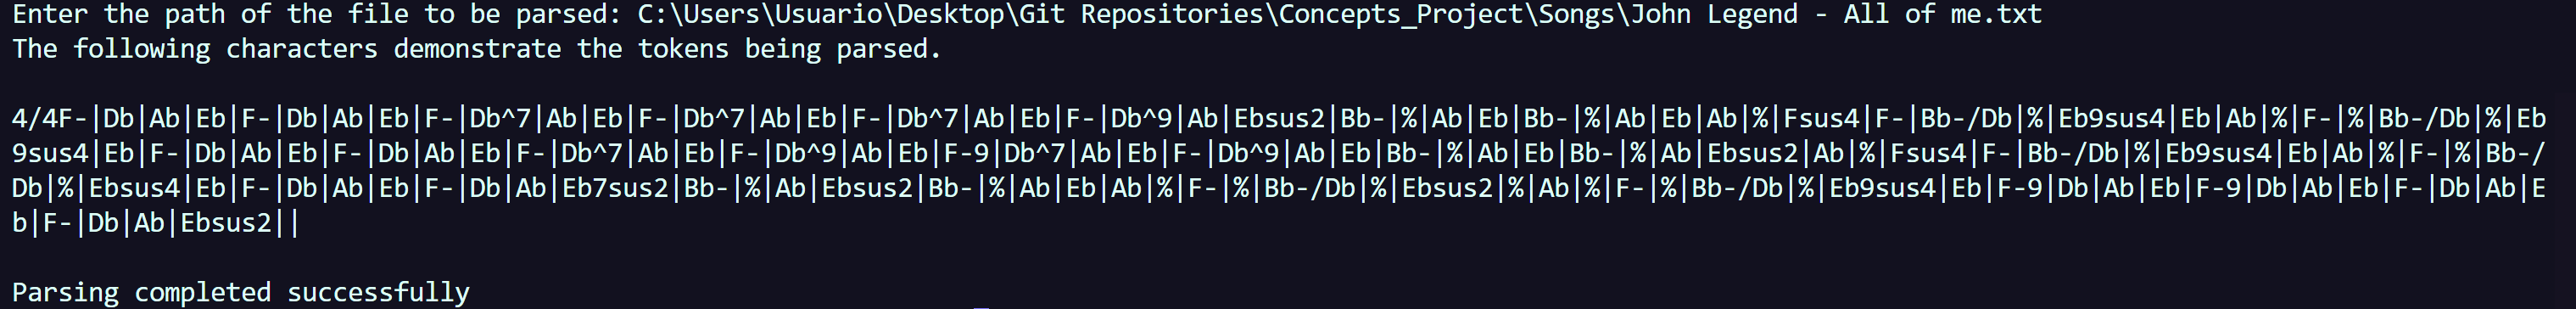
\includegraphics[width=1\textwidth]{Image_AllOfMeParsed.png}
        \caption{Image of outputs on the command line.}
    \end{figure}
    \item \textbf{Test 3}: Luis Miguel - El dia que me quieras.txt
    \begin{figure}[H]
        \centering
        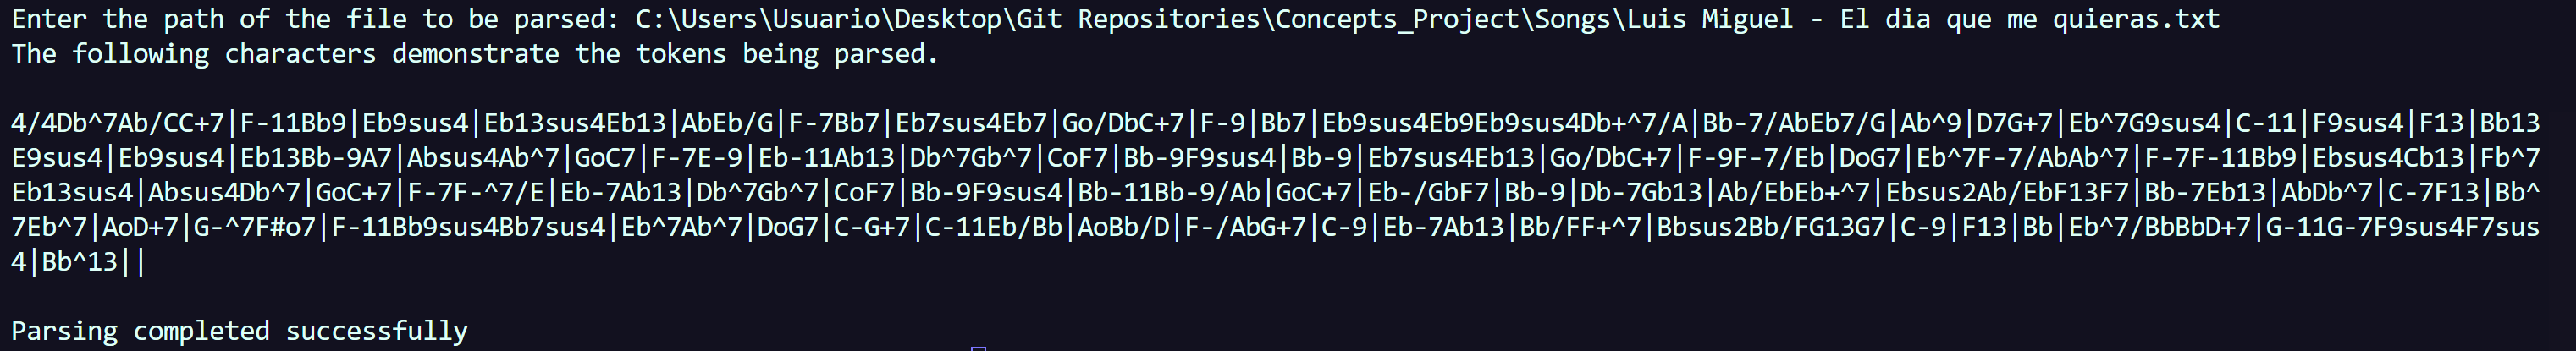
\includegraphics[width=1\textwidth]{Image_ElDiaQueMeQuiera.png}
        \caption{Image of outputs on the command line.}
    \end{figure}
    \item \textbf{Test 4}: Paul McCartney - Uncle Albert / Admiral Halsey (medley).txt
    \begin{figure}[H]
        \centering
        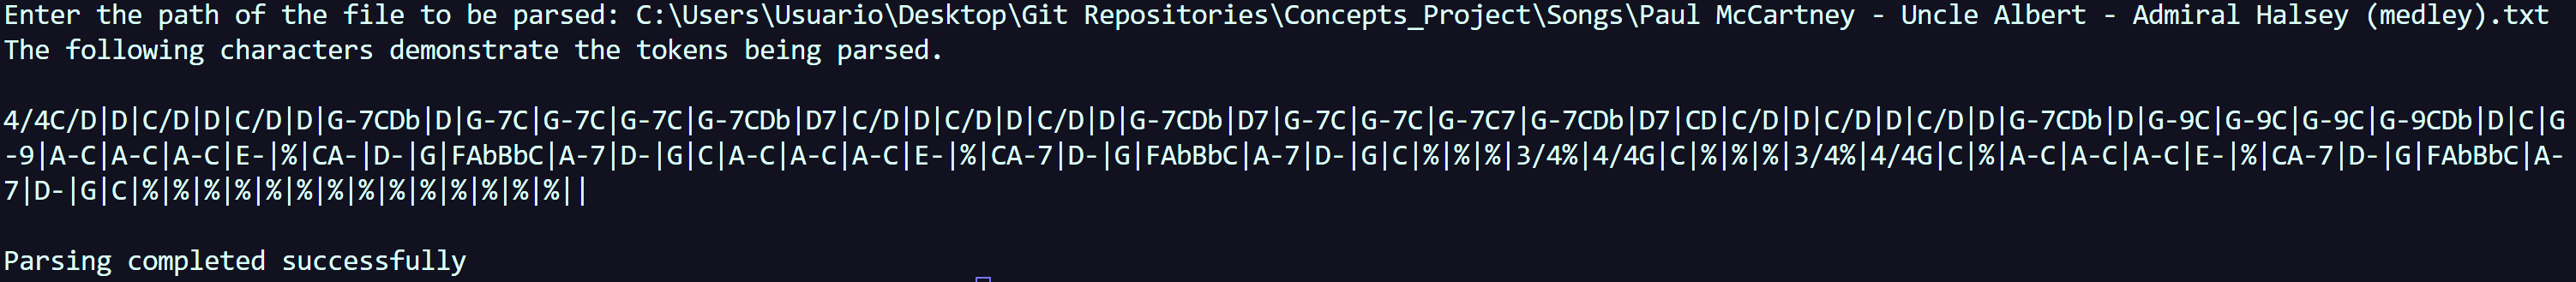
\includegraphics[width=1\textwidth]{Image_AdmiralHalsey.png}
        \caption{Image of outputs on the command line.}
    \end{figure}
    \item \textbf{Test 5}: Queen - Don't stop me now.txt
    \begin{figure}[H]
        \centering
        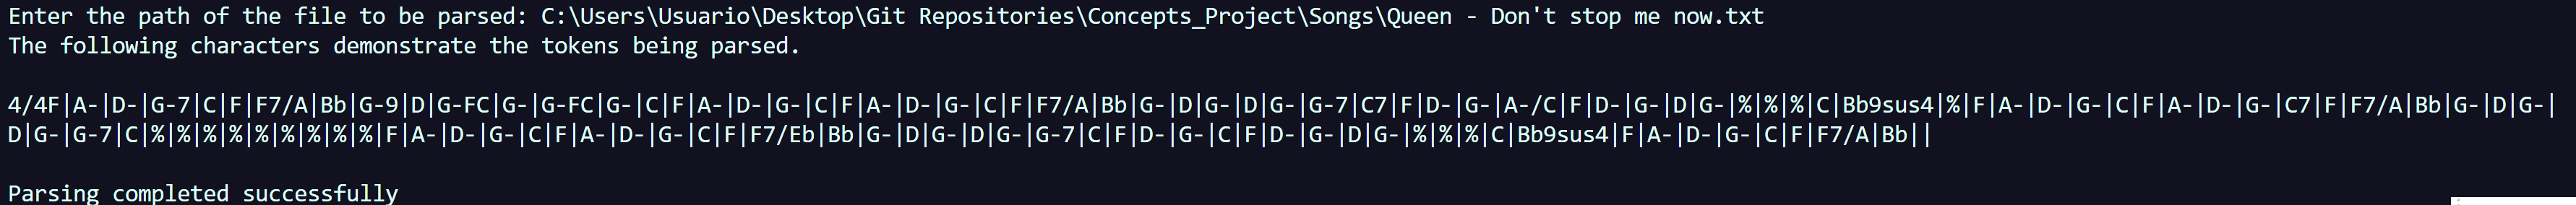
\includegraphics[width=1\textwidth]{Image_DontStopMeNow.png}
        \caption{Image of outputs on the command line.}
    \end{figure}
    \item \textbf{Test 6}: Rocio Durcal - La gata bajo la lluvia.txt
    \begin{figure}[H]
        \centering
        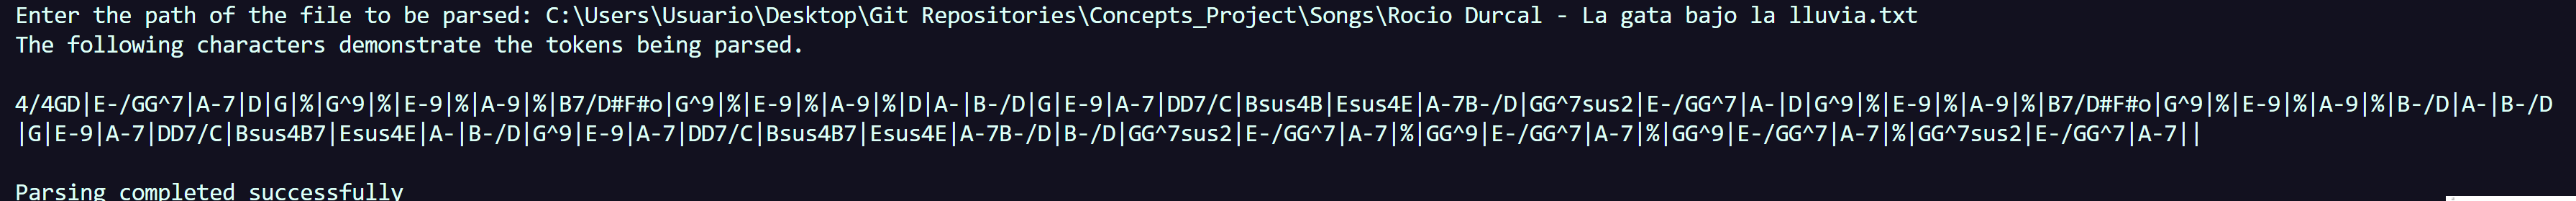
\includegraphics[width=1\textwidth]{Image_LaGataBajoLaLluvia.png}
        \caption{Image of outputs on the command line.}
    \end{figure}
    \item \textbf{Test 7}: Soda Stereo - The musica ligera.txt
    \begin{figure}[H]
        \centering
        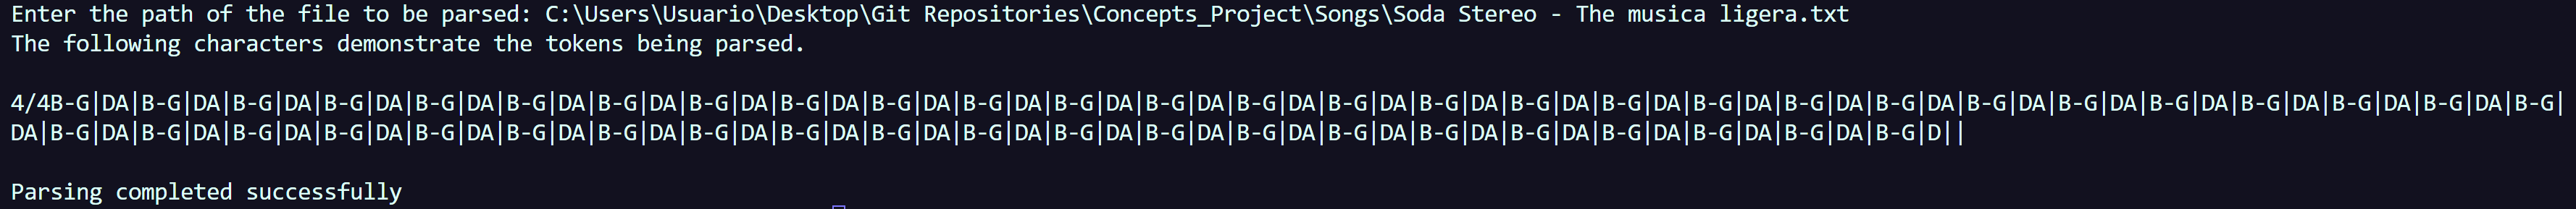
\includegraphics[width=1\textwidth]{Image_DeMusicaLigera.png}
        \caption{Image of outputs on the command line.}
    \end{figure}
\end{itemize}
For the purpose of this deliverable we created a set of \texttt{printf} to demonstrate the behavior of the parsing. The outputs demonstrated in this section are the ones stated here.
\section{Discussion}
This deliverable manages to encompass the desire behavior of a parser, without the full chord calculator which was what was intended for this deliverable. It manages to do so with the use of the functions seen in Section \ref{fig:Functions}, this is demonstrated in Section \ref{fig:Results} with the use of the examples sent by the professor. The examples are in the folder \textbf{Songs} appended with this document. For a more detailed analysis on the functions used to develop the overall functionality please revise the \textbf{Parser.c} file found in the same folder as this document.
\end{document}